\documentclass[12pt]{article}
\usepackage[utf8]{inputenc}
\usepackage[english]{babel}
\usepackage{amsmath, amsthm, amssymb, amsfonts}
\usepackage[top = 3in, left = 1in, right = 1in]{geometry}
\usepackage{hyperref}
\hypersetup{
	colorlinks=true,
	linkcolor=blue,
	filecolor=magenta,      
	urlcolor=blue,
}
\usepackage{tcolorbox}
\usepackage{bm}


% FOR TIKZ
\usepackage{tikz}
\usetikzlibrary{arrows,arrows.meta, shapes.geometric}




% DEFINE NEW COMMANDS AND ENVIRONMENTS
\newcommand{\R}{\mathbb{R}}
\newcommand{\C}{\mathbb{C}}
\newcommand{\N}{\mathbb{N}}
\newcommand{\Q}{\mathbb{Q}}
\newcommand{\Z}{\mathbb{Z}}
\newcommand{\transpose}{\mathsf{T}}

\newcommand{\HRule}{\rule{\linewidth}{0.5mm}} % Defines a new command for the horizontal lines, change thickness here


% DEFINE A PROBLEM Environment
\theoremstyle{definition}
\newtheorem*{prb}{Problem}
\newenvironment{problem}{
\begin{tcolorbox}[colback=blue!5!white,colframe=blue!75!black, parbox = true] \begin{prb}  }{\end{prb}\end{tcolorbox} }


\newenvironment{answer}{\textit{Solution: }\quad }{ \hfill \qedsymbol}



\begin{document}


% TITLE PAGE
%%%%%%%%%%%%%%%%%%%%%%%%%%%%%%%%%%%%%%%%%%%%%%%%%%%%%%
\begin{titlepage}
    
\centering
\textsc{\LARGE Indian Statistical Institute, Kolkata}\\[1.5cm] % Name of your university/college
\textsc{\Large Design of Experiments}\\[0.5cm] % Major heading such as course name
\textsc{\large Assignments in lieu of Semestral Examinations 2020}\\[0.5cm] % Minor heading such as course title

\HRule \\[0.4cm]
\large \textbf{Subhrajyoty Roy}\\
\large \textbf{Roll:  MB1911}\\
\HRule \\[1.5cm]
\normalsize \today

\end{titlepage}


\tableofcontents
\clearpage


% CONTENT FROM HERE
%%%%%%%%%%%%%%%%%%%%%%%%%%%%%%%%%%%%%%%%%%%%%%%%%%
\newgeometry{margin = 1in}

\section{Problem 1}

\begin{problem}
    Eight objects are to be weighed using a weighing balance with two pans. Eight observations will be taken in all, observations being independent and with a constant variance. Give the design matrix of a weighing design which will allow the best linear unbiased estimates of the weights to have the lowest variance across all possible $8 \times 8$ design matrices. The full design matrix must be shown.
\end{problem}


\begin{answer}
	We know that, in the setup of weighing designs, the design which allows the BLUEs to have the lowest possible variance given the number of objects $n$ and number of weighings $p$ is obtained by a Hadamard matrix (or its submatrix containing the columns from Hadamard matrix) of order $n$ (or more). Therefore, to answer the given question, it is enough to obtain a Hadamard matrix of order $8$.
	
	We also know that, if $H_m$ and $H_n$ are two Hadamard matrices of their respective order denoted in subscripts, then $H_m \otimes H_n$, their kronecker product is a Hadamard matrix of order $mn$. Using this, we know that the matrix; $H_8 = H_2 \otimes H_2 \otimes H_2$ is a Hadamard matrix of order $8$, where $H_2$ is a Hadamard matrix of order $2$.

	$$H_2 = \begin{bmatrix}
		1 & 1\\
		1 & -1\\
	\end{bmatrix}$$

	Therefore,

	$$H_2 \otimes H_2 = \begin{bmatrix}
		1 & 1\\
		1 & -1\\
	\end{bmatrix} \otimes \begin{bmatrix}
		1 & 1\\
		1 & -1\\
	\end{bmatrix} = \begin{bmatrix}
		1 & 1 & 1 & 1\\
		1 & -1 & 1 & -1\\
		1 & 1 & -1 & -1\\
		1 & -1 & -1 & 1\\ 
	\end{bmatrix}$$

	And finally,

	$$H_8 = H_2 \otimes (H_2 \otimes H_2) = \begin{bmatrix}
		1 & 1 & 1 & 1 & 1 & 1 & 1 & 1\\
		1 & -1 & 1 & -1 & 1 & -1 & 1 & -1\\ 
		1 & 1 & -1 & -1 & 1 & 1 & -1 & -1\\
		1 & -1 & -1 & 1 & 1 & -1 & -1 & 1\\
		1 & 1 & 1 & 1 & -1 & -1 & -1 & -1\\
		1 & -1 & 1 & -1 & -1 & 1 & -1 & 1\\ 
		1 & 1 & -1 & -1 & -1 & -1 & 1 & 1\\
		1 & -1 & -1 & 1 & -1 & 1 & 1 & -1\\
	\end{bmatrix}$$

	Clearly, $H_8$ as shown above is the design matrix for the weighing design, where, an entry of $+1$ means the object is put into the opposite pan of the weight of the balance, and an entry of $(-1)$ means the object is put into the same pan as the weight of the balance.
\end{answer}


\section{Problem 2}

\begin{problem}
	Let $A$ be the group of residue classes modulo $3$ with elements $0, 1, 2$ and let there be $3$ treatments corresponding to each element of A. For example, corresponding to element $0$, the $3$ treatments are $0_1, 0_2, 0_3$. Consider the $4$ initial blocks:

	$$(1_1, 2_1, 0_2), (1_2, 2_2, 0_3), (1_3, 2_3, 0_1), (0_1, 0_2, 0_3)$$
Check that these initial blocks may be developed to form a BIB design.
\end{problem}

\begin{answer}
	To ensure that the blocks mentioned in the question can be developed to form a BIB design, it is enough to check the following three conditions in view of the theorem regarding "notion of developing a block".

	\begin{enumerate}
		\item Each block $B_j$ contains same number of distinct treatments.
		\item Exactly same number of treatments in all blocks combined belong to each of the $m = 3$ classes.
		\item When all possible pairwise differences between treatments within each blocks are considered together, each possible difference is repeated same number of times. 
	\end{enumerate}

	Now note that, criterion 1 is easily satisfied as each block contains $k = 3$ distinct treatments.

	For criterion 2, it is also easy to see that there are $r = 4$ treatments belonging to each of the class. For example, first block has $1_1, 2_1$, second block has none, third and fourth block each has $0_1$, as treatments from class $1$. Similar for class $2$ and $3$.
	
	Finally, for criterion 3, note that there are $9$ types of differences.
	
	\begin{itemize}
		\item $3$ pure differences, $(1, 1), (2, 2), (3, 3)$.
		\item $6$ mixed differences, $(1, 2), (1, 3), (2, 1), (2, 3), (3, 1), (3, 2)$
	\end{itemize}

	Now, the pure difference can be of value $1, 2$ and the mixed difference can be of value $0, 1, 2$. From each of the first three blocks, we have pure difference of type $i$ of value $1, 2$ from the differences $(2_i - 1_i)$ and $(1_i - 2_i)$ respectively. Each type of mixed difference of value $0$ is obtained from last block, while mixed difference of any nonzero value can be obtained from first three blocks. For instance, the first block gives mixed differences of type $(1, 2)$ and $(2, 1)$ for all nonzero values. Therefore, each possible difference is repeated $\lambda = 1$ time.

	This verifies the above three conditions in order to apply the related theorem to conclude that the given blocks can be developed to form a BIB design with parameters $v = 9, b = 12, r = 4, k = 3, \lambda = 1$.
\end{answer}


\section{Problem 3}

\begin{problem}
	Construct a BIB design by developing the blocks in 2 above and give its parameters.
\end{problem}

\begin{answer}
	We have the initial blocks given as;
	$$B_{1,0} = (1_1, 2_1, 0_2), B_{2, 0} = (1_2, 2_2, 0_3), B_{3,0} = (1_3, 2_3, 0_1), B_{4, 0} = (0_1, 0_2, 0_3)$$

	Since, these blocks are created based on the group of residue class modulo $3$ containing the elements $0, 1, 2$, we can simply obtain the new blocks as;

	$$B_{j,1} = B_{j, 0} + 1 \qquad B_{j,2} = B_{j, 0} + 2 $$
	
	Namely, the final blocks are as follows:

	$$\begin{array}{llll}
		B_{1,0} = (1_1, 2_1, 0_2) 
		& B_{2, 0} = (1_2, 2_2, 0_3)
		& B_{3,0} = (1_3, 2_3, 0_1)
		& B_{4, 0} = (0_1, 0_2, 0_3)\\
		B_{1,1} = (2_1, 0_1, 1_2) 
		& B_{2, 1} = (2_2, 0_2, 1_3)
		& B_{3,1} = (2_3, 0_3, 1_1)
		& B_{4, 1} = (1_1, 1_2, 1_3)\\
		B_{1,2} = (0_1, 1_1, 2_2) 
		& B_{2, 2} = (0_2, 1_2, 2_3)
		& B_{3,2} = (0_3, 1_3, 2_1)
		& B_{4, 2} = (2_1, 2_2, 2_3)
	\end{array}$$

	Clearly, the above design is a BIB design with the parameters; $v = 9, b = 12, r = 4, k = 3, \lambda = 1$.

\end{answer}


\section{Problem 4}

\begin{problem}
	Using the BIB design constructed above, construct a BIB with $v = 9, b = 12, k = 6$.
\end{problem}

\begin{answer}
	Note that, there are in total $v = 9$ treatments in above BIB design and each block is of size $k = 3$. Now to create another BIB design with block size $k = (9-3) = 6$, it is simply enough to create block $B_j'$ corresponding to each block $B_j$ such that it contains the complementary treatments, i.e. the treatments which do not appear in the block $B_j$. Essentially, this amounts to creation of a complementary block design.

	The blocks for this new BIB design is as follows:

	$$\begin{array}{llll}
		B_{1,0}' = (1_2, 1_3, 2_2, 2_3, 0_1, 0_3) 
		& B_{2, 0}' = (1_1, 1_3, 2_1, 2_3, 0_1, 0_2)\\
		B_{3,0}' = (1_1, 1_2, 2_1, 2_2, 0_2, 0_3)
		& B_{4, 0}' = (1_1, 1_2, 1_3, 2_1, 2_2, 2_3)\\
		& \\
		B_{1,1}' = (2_2, 2_3, 0_2, 0_3, 1_1, 1_3) 
		& B_{2, 1}' = (2_1, 2_3, 0_1, 0_3, 1_1, 1_2)\\
		B_{3,1}' = (2_1, 2_2, 0_1, 0_2, 1_2, 1_3)
		& B_{4, 1}' = (0_1, 0_2, 0_3, 2_1, 2_2, 2_3)\\
		& \\
		B_{1,2}' = (0_2, 0_3, 1_2, 1_3, 2_1, 2_3) 
		& B_{2, 2}' = (0_1, 0_3, 1_1, 1_3, 2_1, 2_2)\\
		B_{3,2}' = (0_1, 0_2, 1_1, 1_2, 2_2, 2_3)
		& B_{4, 2}' = (0_1, 0_2, 0_3, 1_1, 1_2, 1_3)\\
		& \\
	\end{array}$$

	These blocks consitute a BIB design with parameters $v = 9, b = 12, k = 6, r = 8, \lambda = 5$.

\end{answer}


\section{Problem 5}

\begin{problem}
	You are to plan an experiment to study the effect of $2$ different culture-mediums and $3$ different experiment times on the growth of a particular virus. Each day, six observations can be taken under identical conditions and the experiment is to be continued for $3$ days. Suggest a design for this factorial experiment.
\end{problem}

\begin{answer}
	We see that, there are $2$ different culture mediums and $3$ different experiment times, thereby constituting a total of $2 \times 3 = 6$ factor combinations. Let, the $6$ treatment combination be denoted as $\left\{ 00, 01, 02, 10, 11, 12 \right\}$ where combination $ab$ means level $a$ of culture medium applied for level $b$ of experiment time.
	
	Now, it is also given that each day only $6$ observations can be taken under identical conditions, and it is implied that the conditions may vary from day to day. Therefore, the particular day on which the experiment is performed consitutes a blocking factor. Hence, in the mathematical model explaining the responses, there will be terms like $\tau_i$ (the effect of $i$-th level of culture), $\alpha_j$ (the effect of $j$-th level of experiment times), $(\tau\alpha)_{ij}$ (interaction of the factors) and $\beta_k$, a blocking factor. To ensure estimability of the main effects and the interaction effects, it is required that each of the treatment combination appears in a single block atleast once (because of connectedness), and to ensure all normalized contrasts are estimated with most precision, all blocks should be similar in the sense of which factor combinations they contain and how many (because of equireplication). Also, if we ensure orthogonality so that the factor effects do not confound with the block effects and analysis of the design is easier to deal with, then the incidence matrix $N \propto rk^{T}$ matrix (because of both orthogonality and connectedness). 

	Therefore, a suitable design for the above scenario would be to use \textbf{Randomized Block Design} (RBD) where each day, each of the factor combination is applied once, in a random order to randomly assigned experimental units.

\end{answer}

\section{Problem 6}

\begin{problem}
	In the context of a $3 \times 2 \times 4$ factorial experiment with factors $F_1$, $F_2$ and $F_3$, write down the expression for the contrasts belonging to the main effect $F_2$ and interaction $F_1F_2F_3$.
\end{problem}

\begin{answer}
	Let, us consider the levels of the factors starting from $0$, and be denoted by string (or sequence) of numerals in the order of $F_1, F_2$ and $F_3$ respectively.

	We consider the vector of treatment effects as;

	$$\tau = \left( \tau(000), \dots \tau(003), \tau(010), \dots \tau(013), \tau(100), \dots \tau(213) \right)^{T}$$

	which is a vector of length $(3 \times 2 \times 4) = 24$.

	Now, let us consider the orthogonal helmert contrasts (without the normalizing constants) for each of the factors as follows:

	$$\begin{array}{lll}
		P_{F_1} = \begin{bmatrix}
			1 & -1 & 0\\
			1 & 1 & -2\\
		\end{bmatrix};
		& 
		P_{F_2} = \begin{bmatrix}
			1 & -1
		\end{bmatrix};
		&
		P_{F_3} = \begin{bmatrix}
			1 & -1 & 0 & 0\\
			1 & 1 & -2 & 0\\
			1 & 1 & 1 & -3\\
		\end{bmatrix}
	\end{array}$$

	Therefore, the contrasts related to the main effect $F_2$ is simply given by;

	\begin{align*}
		P^{010}\tau 
		& = \left[\bm{1}_{3} \otimes P_{F_2} \otimes \bm{1}_{4}\right]\tau \\
		& = \left[\begin{bmatrix}
			1 & -1 & 1 & -1 & 1 & -1
		\end{bmatrix} \otimes \bm{1}_4\right] \tau \\
		& = \begin{bmatrix}
			\underbrace{1 \dots}_{4 \text{ times}} 
			& \underbrace{(-1) \dots}_{4 \text{ times}}
			& \underbrace{1 \dots}_{4 \text{ times}} 
			& \underbrace{(-1) \dots}_{4 \text{ times}}
			& \underbrace{1 \dots}_{4 \text{ times}} 
			& \underbrace{(-1) \dots}_{4 \text{ times}}
		\end{bmatrix} \tau\\
	\end{align*}

	\begin{align*}
		\therefore P^{010}\tau	
		& = \tau(000) + \dots +\tau(003) - \tau(010) - \dots - \tau(013) + \ldots - \tau(210) - \dots - \tau(213)\\
		& = \sum_{i = 0}^{1} \sum_{j = 0}^{4} \left[ \tau(i,0,j) - \tau(i, 1, j) \right]
	\end{align*}

	Now, the normalizing constant can be easily obtained by noting that there are $24$ such terms, and each coefficient is either $(+1)$ or $(-1)$. Hence, the contrast belonging to $F_2$ is given by $$\dfrac{1}{\sqrt{24}} \sum_{i = 0}^{1} \sum_{j = 0}^{4} \left[ \tau(i,0,j) - \tau(i, 1, j) \right]$$

	For the interaction $F_1F_2F_3$, we consider;

	\begin{align*}
		P^{111}\tau
		& = \left[ P_{F_1} \otimes P_{F_2} \otimes P_{F_3} \right] \tau \\
		& = \left( \begin{bmatrix}
			1 & -1 & -1 & 1 & 0 & 0\\
			1 & -1 & 1 & -1 & -2 & 2\\
		\end{bmatrix} \otimes 
		\begin{bmatrix}
			1 & -1 & 0 & 0\\
			1 & 1 & -2 & 0\\
			1 & 1 & 1 & -3\\
		\end{bmatrix} \right) \tau\\
	\end{align*}

	The first row of the resulting kronecker product is, $$(1, -1, 0, 0, -1, 1, 0, 0, -1, 1, 0, 0, 1, -1, 0, 0, \underbrace{0, \dots 0}_{8 \text{ times}})$$

	which multiplied with the $\tau$ vector gives the first contrast for the interaction $F_1F_2F_3$. Then, we can simply normalize this contrast as $l^T\tau / \Vert l \Vert$, where $l$ is a row of the kronecker product.

	So, finally $6$ treatment contrasts corresponding to the interaction effect $F_1F_2F_3$ are simply given as follows:

	\begin{align*}
		L_1 & = \dfrac{1}{2\sqrt{2}} \Big(  \tau(000) - \tau(001) - \tau(010) + \tau(011) - \tau(100) + \tau(101) + \tau(110) - \tau(111)  \Big) \\
		L_2 & = \dfrac{1}{2\sqrt{6}} \Big( \tau(000) + \tau(001) - 2\tau(002) - \tau(010) - \tau(011) + 2\tau(012) \\
		& \qquad \qquad  - \tau(100) - \tau(101) + \tau(102) + \tau(110) + \tau(111) - 2\tau(112) \Big)\\
		L_3 & = \dfrac{1}{4\sqrt{3}} \Big(
			  \tau(000) + \tau(001) + \tau(002) - 3 \tau(003)
			- \tau(010) + \tau(011) + \tau(012) - 3 \tau(013) \\
		& \qquad \qquad
			- \tau(100) + \tau(101) + \tau(102) - 3 \tau(103) 
			+ \tau(110) + \tau(111) + \tau(112) - 3 \tau(113) 
		\Big)
	\end{align*}

	\begin{align*}
		L_4 & = \dfrac{1}{2\sqrt{6}} \Big(
			 \tau(000) - \tau(001) 
			- \tau(010) + \tau(011)
			+ \tau(100) - \tau(101)
			- \tau(110) + \tau(111)\\
			& \qquad \qquad
			-2 \tau(100) + 2\tau(101)
			+ 2 \tau(110) - 2\tau(111)
			\Big)\\
		L_5 & = \dfrac{1}{6\sqrt{2}} \Big(
			\tau(000) + \tau(001) - 2\tau(002)
			- \tau(010) - \tau(011) + 2\tau(012)\\
			& \qquad \qquad
			+ \tau(100) + \tau(101) - 2\tau(102)
			- \tau(110) - \tau(111) + 2\tau(112)\\
			& \qquad \qquad
			-2\tau(200) -2 \tau(201) +4 \tau(202)
			+ 2\tau(210) + 2\tau(211) - 4\tau(212)
			\Big)\\
		L_6 & = \dfrac{1}{12} \Big(
			\tau(000) + \tau(001) + \tau(002) - 3\tau(003)	
			- \tau(010) - \tau(011) - \tau(012) + 3\tau(013)\\
			& \qquad
			+ \tau(100) + \tau(101) + \tau(102) - 3\tau(103)	
			- \tau(110) - \tau(111) - \tau(112) + 3\tau(113)\\	
			& \qquad
			-2\tau(200) -2 \tau(201) -2 \tau(202) +6\tau(203)	
			+ 2\tau(210) + 2\tau(211) + 2\tau(212) - 6\tau(213)
		\Big)
	\end{align*}

\end{answer}


\section{Problem 7}

\begin{problem}
	Consider the $3 \times 4$ factorial arranged in a design $d$ with $12$ blocks, as shown below: (Blocks are shown as columns)

	$$
	\begin{array}{llllllllllll}
		00 & 00 & 00 & 01 & 01 & 01 & 02 & 02 & 02 & 03 & 03 & 03\\
		11 & 12 & 13 & 10 & 12 & 13 & 10 & 11 & 13 & 10 & 11 & 12\\
		22 & 23 & 21 & 23 & 20 & 22 & 21 & 23 & 20 & 22 & 20 & 21\\
	\end{array}
	$$
	Derive the $C$ matrix of $d$ and show that $d$ has OFS and balance.
\end{problem}


\begin{answer}
	In this design $d$, there are $12$ treatment combinations, each replicated $3$ times, and block sizes are all equal to $3$. 

	$$\therefore C_d = r I_{12} - \dfrac{1}{k} N_d N_d^T = 3 I_{12} - \dfrac{1}{3} N_d N_d^{T}$$

	where $I_n$ denotes the identity matrix of order $n \times n$.

	Now, $(N_d N_d^T)_{ii'} = \sum_{j = 1}^{12} n_{ij}n_{i'j}$, i.e. the number of blocks in which both treatment combination $i$ and treatment combination $i'$ occurs. Clearly, $(N_d N_d^T)_{ii} = 3$ for any treatment combination $i$. 

	To find the non-diagonal element, we consider several cases:

	\begin{enumerate}
		\item Consider, $i = (a,b), i' = (a, c)$, where $b \neq c$. That means, the treatment combinations $i$ and $i'$ has the level of first factor in common. Notice that, in each of the block, the each of the levels of the first factor is taken only once, hence such $(N_d N_d^T)_{ii'} = 0$.
		\item Consider, $i = (a,b), i' = (c, b)$, where $a \neq c$. That means, the treatment combinations $i$ and $i'$ has the level of second factor in common. Clearly, by similar logic, $(N_d N_d^T)_{ii'} = 0$ as the treatment combinations in each block has different levels of second factor.
		\item Consider, $i = (a, b), i' = (c, d)$, where $a \neq c$, and $b \neq d$. In this case, $(N_d N_d^T)_{ii'} = 1$ as every pair of combinations come exactly once considering all blocks.
	\end{enumerate}

	$$\therefore N_d N_d^T = 3 I_{12} + (J_3 - I_3) \otimes (J_4 - I_4)$$

	where $J_n$ is the $n \times n$ matrix with all entries equal to $1$.

	So, we obtain;

	\begin{align*}
		C_d 
		& = 3I_{12} - \dfrac{1}{3} \left[ 3 I_{12} + (J_3 - I_3) \otimes (J_4 - I_4) \right] \\
		& = 3 I_{12} - \dfrac{1}{3} \left[ 3I_{12} + J_{12} - I_3 \otimes J_4 - J_3 \otimes I_4 + I_{12} \right]\\
		& = 3 I_{12} - \dfrac{1}{3} \left[ 4I_{12} + J_{12} - I_3 \otimes J_4 - J_3 \otimes I_4  \right]\\
		& = \dfrac{5}{3} I_{12} + \dfrac{1}{3} I_3 \otimes J_4 + \dfrac{1}{3} J_3 \otimes I_4 - \dfrac{1}{3} J_{12}\\
	\end{align*}

	Clearly, note that the given design $d$ is connected, so to show that $d$ has OFS and balance, it is enough to show that the matrix $C_d$ has the following form:

	\begin{equation}
		C_d = \sum_{x \in \Omega} a(x) (P^x)' (P^x)
		\label{eqn:Cd-mat}
	\end{equation}

	We also know that,

	$$(P^x)'(P^x) = \otimes_{i=1}^{n} (P^{x_i})'(P^{x_i})$$

	where;

	$$(P^{x_i})'(P^{x_i}) = \begin{cases}
		I_{s_i} - \dfrac{1}{s_i} J_{s_i} & \text{ if } x_i = 1\\
		\dfrac{1}{s_i} J_{s_i} & \text{ if } x_i = 0\\
	\end{cases}$$

	Now, as there are two factors, we consider $P^{10}, P^{01}$ and $P^{11}$ only, which yields,

	$$
	P^{10} = \dfrac{1}{4} (I_3 - \dfrac{1}{3} J_3) \otimes J_4,
	\quad 
	P^{01} = \dfrac{1}{3} J_3 \otimes (I_4 - \dfrac{1}{4} J_4),
	\quad
	P^{11} = (I_3 - \dfrac{1}{3} J_3) \otimes (I_4 - \dfrac{1}{4} J_4)
	$$

	Continuing with the expression of $C_d$, we get;

	\begin{align*}
		C_d
		& = \dfrac{5}{3} \left[ I_{12} - \dfrac{1}{3} J_3 \otimes I_4 - \dfrac{1}{4} I_3 \otimes J_4 + \dfrac{1}{12} J_{12} \right] + \dfrac{8}{3} \left[ \dfrac{1}{3} J_3 \otimes I_4 - \dfrac{1}{12} J_{12} \right] \\
		& \qquad \qquad + 3 \left[ \dfrac{1}{4} I_3 \otimes J_4 - \dfrac{1}{12}J_{12} \right] \\
		& = \dfrac{5}{3} P^{11} + \dfrac{8}{3} P^{01} + 3 P^{10}\\
	\end{align*}

	which is of the form as specified in \eqref{eqn:Cd-mat}. This completes the proof that the design $d$ has OFS and Balance.


\end{answer}


\section{Problem 8}

\begin{problem}
	Construct an orthogonal array $OA(9, 4, 3, 2)$ starting from $2$ mutually orthogonal Latins squares of order $3$.
\end{problem}

\begin{answer}
	We start with the following $2$ MOLS with order $3$.

	$$L_1 = 
	\begin{bmatrix}
		0 & 1 & 2\\
		1 & 2 & 0\\
		2 & 0 & 1\\
	\end{bmatrix}
	\qquad  \qquad
	L_2 = \begin{bmatrix}
		0 & 1 & 2\\
		2 & 0 & 1\\
		1 & 2 & 0\\
	\end{bmatrix}
	$$

	Now, the resulting orthogonal arrays can simply be obtained by writing the columns of above latin squares top to bottom in a single column and add two more columns to it, one being $(0, \dots 0, 1, \dots 1, 2 \dots 2)$ each being repeated $3$ times, and another column being $(0, 1, 2)$ repeated for $3$ times.

	Therefore, we finally get the orthogonal array as follows:

	$$
	\begin{matrix}
		0 & 0 & 0 & 0 \\
		1 & 2 & 0 & 1 \\
		2 & 1 & 0 & 2 \\
		1 & 1 & 1 & 0 \\
		2 & 0 & 1 & 1 \\
		0 & 2 & 1 & 2 \\
		2 & 2 & 2 & 0 \\
		0 & 1 & 2 & 1 \\
		1 & 0 & 2 & 2 \\
	\end{matrix}
	$$

	Clearly, this is an orthogonal array $OA(9, 4, 3, 2)$, since it is a $9 \times 4$ size array with $3$ symbols $0, 1, 2$ such that, in every $9 \times 2$ subarray all ordered $2$ tuples appear exactly once as rows.

\end{answer}


\section{Problem 9}

\begin{problem}
	What is a main effect plan, or equivalently, a Resolution III plan?
\end{problem}

\begin{answer}
	A main effect plan or Resolution III plan is a fractional factorial experiment plan where the main effects of all the factors are not confounded with each other, but main effects are confounded with the two way or higher order interactions, as well as two way or higher order interaction effects can be confounded with each other.
	
	In such plan, the contrasts related to the main effects are estimable under the assumption that all two order or higher order interactions between two or more factors are absent in the model.

	Resolution III designs can be very useful in the situations where there are relatively many factors but only a few of them are expected to be important.
\end{answer}


\section{Problem 10}

\begin{problem}
	From the $OA(9, 4, 3, 2)$ constructed in question 8 above, obtain a $9$-run main effect plan for a $3^4$ factorial.
\end{problem}

\begin{answer}
	To obtain a $9$-run main effect plan for $3^4$ factorial, i.e. to constract a $3^{4-2}$ plan so that all main effects are estimable, one can simply consider the rows of the orthogonal array, each giving one combination of the factors to be experimented with the unit. We may assume the absence of all two or higher order interactions, i.e. a Resolution III plan, and as $R = 3 \geq (t + 1)$, for $t = 2$, in $OA(9, 4, 3, 2)$, the necessary theorem applies as quoted below:

	\textit{
		 ``Let $d$ be an $s^{n-k}$ plan of resolution $R$. If $R \geq t + 1$, then the treatment combinations included in $d$, when written as rows, form an $OA(s^{n-k}, n, s, t)$."
	}

	Therefore, the treatment combinations for the $9$-run plans are given as;

	$$
	\left[  
		0000, 1201, 2102, 1110, 2011, 0212, 2220, 0121, 1022
	\right]
	$$

	where the sequence $(i_1i_2i_3i_4)$ denotes the treatment combination where the first factor is applied at $i_1$-th level, second factor is applied at $i_2$-th level, third factor is applied at $i_3$-th level and last factor is applied at $i_4$-th level.

\end{answer}


\vspace*{1in}

\begin{center}
	{\Large\textit{Thank you}}
	\vspace*{0.25in}\\
	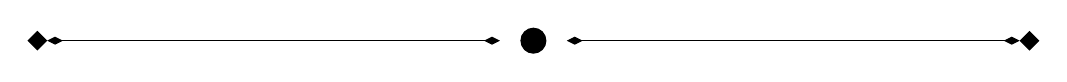
\begin{tikzpicture}[scale = 3]
		\node (a) at (0,0) {};
		\node (b) at (2,0) {};
		\draw[fill] (2.1, 0) circle (1.5pt);
		\node[draw, diamond, fill = black, scale = 0.5] at (0,0) {};
		\node (d) at (2.2,0) {};
		\node (e) at (4.2,0) {};
		\node[draw, diamond, fill = black, scale = 0.5] at (4.2,0) {};
		\draw [{Diamond}-{Diamond}] (a.east) -- (b.west);
		\draw [{Diamond}-{Diamond}] (d.east) -- (e.west);
	\end{tikzpicture}
\end{center}


\end{document}

